\subsubsection{Final Fantasy}

\paragraph{Outline}

Strat ME clone. Unbalanced map, West > East, easier to defend, better bottlenecks, better proximity towards the other 2 regions (above 2 + North). You can win vs a robot with 10 second picks, gameplay and luck on leftovers matters more. North is either safe +4 bonus to soft counter late the SW, or combo +5 that runs the whole map. +5s in general are extremely strong, sometimes unsuspected, and win games due to their better borders.

\url{https://www.youtube.com/watch?v=MwQKbpBR4iY} 4x4, neutrals 2/2, wastelands 7/12, base: +5

\paragraph{Map Dynamics}

\url{https://imgur.com/JDjlxti} old picture

\begin{figure}[H]
  \centering
  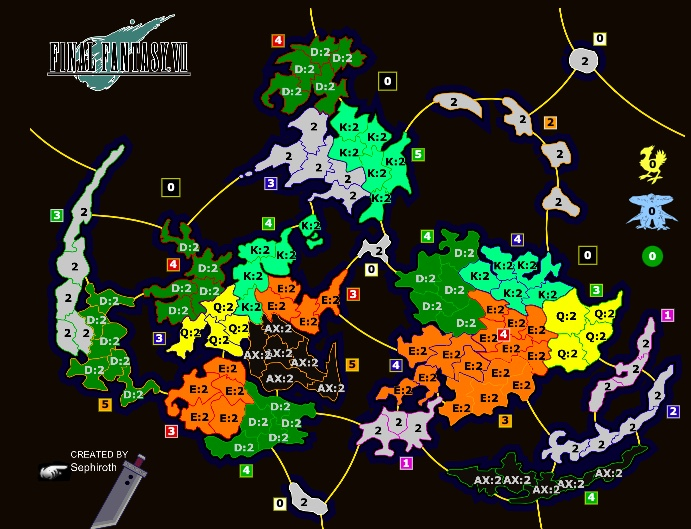
\includegraphics[width=0.8\textwidth]{Images/1800ff7.jpg}
  \caption{Bonus Win Rates for Games with Overall Winner Rating >=1800 in Final Fantasy VII(n=397) (AX>D>K>Q>E>-).}
  \label{ff7_1800}
\end{figure}

Once upon a time I played this \href{https://www.warzone.com/MultiPlayer?GameID=38090471}{game} and ever since them vetoed the shit out of this template. So be warned, my opinion on it, isn't thorough, nor objective, nor professional.
\\
\\
Generally speaking, West Continent > East Continent > North Continent. Also generally speaking, bigger bonuses are better? The Win Rates depict to an astonishing match.
\begin{itemize}
    \item AX > 60\% Win Ratio.
    \begin{enumerate}
        \item Central orange +5 has a ridiculous 70\% WR in 69 games, but requires specific setup such as a) Picking it for a safe region overall \href{https://www.warzone.com/MultiPlayer?GameID=37701672}{here}, b) for FTB blue +3 \href{https://www.warzone.com/MultiPlayer?GameID=34110306}{here}, c) for +5 combo \href{https://www.warzone.com/MultiPlayer?GameID=33927948}{here}, d) for a +4 combo \href{https://www.warzone.com/MultiPlayer?GameID=29946478}{here} and more. It's strength is in it's position. 
        \item Green island +4 (Mideel Island) all the way south, is very very situational, don't let it's WR confuse you, it has 15W in 25G in a 387G pool. It has 2-3 purposes. a) be a safe +4 bonus for a setup where you want to attack your opponent on T4-T5 like \href{https://www.warzone.com/MultiPlayer?GameID=38755207}{here}. and \href{https://www.warzone.com/MultiPlayer?GameID=32885604}{here} b) Be a sneaky counter to the Eastern Continent like \href{https://www.warzone.com/MultiPlayer?GameID=33185191}{here} and \href{https://www.warzone.com/MultiPlayer?GameID=29832639}{here} (lol the games look identical) c) Be a safe bonus if you plan on doing 12combo 3 safe 456 cover or 12 safe 3456 cover or if you want to bait your opponent into over-committing in a region with multiple picks and go hunt with army advantage. For example \href{https://www.warzone.com/MultiPlayer?GameID=37715740}{here}, it does all of those at the same time. You basically need to setup contact later, whether that's on Turns 4-5, or even later if the opponent mindlessly expands like \href{https://www.warzone.com/MultiPlayer?GameID=28354694}{here}.
    \end{enumerate}
    \item D > 55\% Win Ratio.
    \begin{enumerate}
        \item All of the +4 Bonuses in this list are good either as combos or as solo picks, depending on distribution. For solo pick, you opt for later contact and accompany with centralized picks in other bonuses. For combos, you want earlier contact. All of those generally provide you with some benefits, as for example the Green +4 south and the one east have great proximity to major income regions. The red +4 north is very safe for slower picksets, and the red +4 west combos great with the +5 and a potential +3 FTB, while also having great defensive borders.
    \end{enumerate}
    \item After checking a couple of games for every other bonus, I realised that a couple of good players were just styling on everyone else that blindly picked FTBs, so don't have anything to add, bonuses can be situationally good everywhere, don't see the orange sea east and avoid picking it. The general issue with the region is it's vulnerable from everywhere and you'd have to guess where to expand towards.
\end{itemize}

\paragraph{Picking Logic}

It's a 3 spawns WR template, there's maybe five different ideas and with good intuition you can pick one of those five within seconds of the game starting and get a fine position. Not that this means you can find perfect picks this fast, but you can make very decent picks very fast, gameplay and luck on leftovers matter way more. You can choose to optimize picks for longer than 30 seconds but I advice you not to, contrary to what a lot of players thought about me, I just threw picks on pattern a good 99\% of the time and they got me to 2000 rating.
\\
\\
So, 3 spawns WR template, we've got:

\begin{enumerate}
    \item 1/2 + 3 safe + 456 vs 1/2 + 3456 vs 1 + 2/3 + 4/5/6.
    \begin{itemize}
        \item So generally I would advise you to absolutely never do 1/2 combo and 3456 another region, like \href{https://www.warzone.com/MultiPlayer?GameID=36661144}{here}. It can of course work, but it is a boring, unimaginative way of picking where you downgrade the game to whether or not you win on T2/T3. Chances are you'll lose. The other grand downside of this is that if you split with your opponent the 1/2 combo, you end up with 2 picks in the 3456 cluster vs 1 from your opponent -> you lose.
        \item 12 + 3456 can work in a fancier way against players against players that will pick 1/2 + 3 safe + 456 like \href{https://www.warzone.com/MultiPlayer?GameID=34380052}{here}, where Castel plays around splitting his 1/2 combo and getting one of 1/2, 3 and a cover east, but gets 1/2/3 -> loses on picks. (Another thing that can work in these situations if you have Jacob's balls is doing 1/2/3 where you expect the enemy to do 4/5/6).
        \item the 1 + 2/3 + 4/5/6 strat heavily gambles on getting first pick - assumes your opponent won't have the same first pick. Nevertheless it can work, it's just not my cap of tea. For example \href{https://www.warzone.com/MultiPlayer?GameID=33889327}{here} 1 coverage, 2/3 combo +5, 456 coverage
    \end{itemize}
    \item 1/2, 3/4, 5/6 combos and mixing things up if 1 is stronger than 2.
    \begin{itemize}
        \item \href{https://www.warzone.com/MultiPlayer?GameID=40838281}{here}, first pick controls 2 FTBs, we both place the other territory on 3 instead of 2, to combo 1/3. The reason is if my opponent is blind and cannot see why "North Corel" is a must first pick, Octane has 50\% chance to get both his 1st and 2nd pick (with his 2nd being really strong east). I just threw my 2 north, but made picks in 5 minutes, don't expect much. You can see the pattern however, 1/3 FTB, 2/4 FTB, 5/6 Combo, 5 as safe income, 6 to cover 5 + safe income itself. 6 in the south +4 because it likely comes in sets of losing 1st pick, and has a path to the blue +3 west. Similarly, \href{https://www.warzone.com/MultiPlayer?GameID=32067072}{here} Rufus' 1st pick is quite obviously a lot better than his 3rd pick for that slow combo.
    \end{itemize}
    \item +3 FTB distributions
    \begin{itemize}
        \item The "3/4/5" approach, \href{https://www.warzone.com/MultiPlayer?GameID=38505036}{here}, \href{https://www.warzone.com/MultiPlayer?GameID=38486921}{here}, I find another combo, 3/4/5 FTB, If I get 1/2 + one of 345 I'm so good at this game. If I get 126 my 6 better soft cover that region else I'm griefing. 
        \item The "recognising the +3 FTB isn't worth my time, example \href{https://www.warzone.com/MultiPlayer?GameID=34604299}{here}, that south +3 FTB is weak, Crazy reaches contact on T4 down 5 income with a position that's about to collapse within 2 turns. Another example, \href{https://www.warzone.com/MultiPlayer?GameID=32067072}{here}, there's a +3 FTB west and a +3 FTB east. Hergul covers 1/2 west, 3/5 east in plans of countering it, but on Turn 3 he has to make a guess as to where Rufus can be, and if he is wrong and sends a stack to the wrong direction, the tempo loss equals defeat. By Turn 6, you can see one person is expanding with a stack towards his opponent and the other is listening to Maroon 5 oblivious. That's a very important downside of FTBs, when they don't control the entire map, in that, as the person that picked them, you play blindfolded. As the person that didn't pick them, you can literally premove turns 1-6 because you don't have to take a risk in where to expand, you kind of know the opponent is there, build stack in that direction and vamos. Same for +4 FTB.
    \end{itemize}
    \item +4 FTB distributions
    \begin{itemize}
        \item I dare say they aren't as good as you may thing, like it depends. \href{https://www.warzone.com/MultiPlayer?GameID=37300392}{Here} for example dco gets lucky to reach 13 by end of T3, without that he is so behind I'm not sure he can win, though Octane overextends not expecting the solo +5 north.
        \item Another example \href{https://www.warzone.com/MultiPlayer?GameID=32348809}{here}, the +4 FTB is so slow to reach contact west, that by Turn 5 We Ride! has more income. 
        \item \href{https://www.warzone.com/MultiPlayer?GameID=26914947}{Another example} where it actually works, it's a wastelanded +4 FTB though.
    \end{itemize}
    \item solo +4s 123 and 456 cover
    \begin{itemize}
        \item Check the games in the map dynamics for the bonus "Mideel Island". For example \href{https://www.warzone.com/MultiPlayer?GameID=38755207}{here} the 2 solo +4s in 2/3 are the bread and butter of the position, while \href{https://www.warzone.com/MultiPlayer?GameID=29556052}{here} you pick in a way that you surround your opponent's expansion zones and catch them off-guard on Turns 5-6 when they mindlessly expand. (but always risk not getting those solo pick +4s due to the WR gods sleeping).
    \end{itemize}
    \item combo +5
    \begin{itemize}
        \item \href{https://www.warzone.com/MultiPlayer?GameID=37386828}{north +5}, \href{https://www.warzone.com/MultiPlayer?GameID=34604299}{north +5 again}. pay attention at how if you go for a combo +5, you need spawns that won't have neighbours T1-T3, as you don't want to get eliminated in your cover spawn when you invest into expanding. \href{https://www.warzone.com/MultiPlayer?GameID=34553678}{north +5 again}, \href{https://www.warzone.com/MultiPlayer?GameID=33361193}{west +5}, \href{https://www.warzone.com/MultiPlayer?GameID=32562403}{west +5 again}
    \end{itemize}
\end{enumerate}

\paragraph{Gameplay}
% early, mid, cards

I generally would suggest playing some games to test things out and your limits, FF7 is a tricky map, where you can pivot very easily due to how bonuses are formed. For example in \href{https://www.warzone.com/MultiPlayer?GameID=32756346}{this game}, alex gets a 12vs11 income up in armies position end of Turn 4 and is about to nuke that +3 bonus south which it's crucial to realize from Buns' POV you cannot and must not defend. You have the option to abandon the region with a blockade at the very left edge later on, you suspect the south Green +4 by the opponent and you also have nothing to protect in the region, alex over-commits in the region but has horrific tempo across Turns 4-6 and practically hopes for a miracle elimination. And he does get the 50-50 priority on Turn 7, but still the game end of Turn 7 positionally is winning for Buns, even if he is down 30 armies, as those armies are on vacation at Honolulu.
\\
\\
On a last note, this follows the very same thing I said on map dynamics and is an extension to pivoting. West > East > North, with reference to Figure \ref{ff7_proximity}.

\begin{figure}[H]
  \centering
  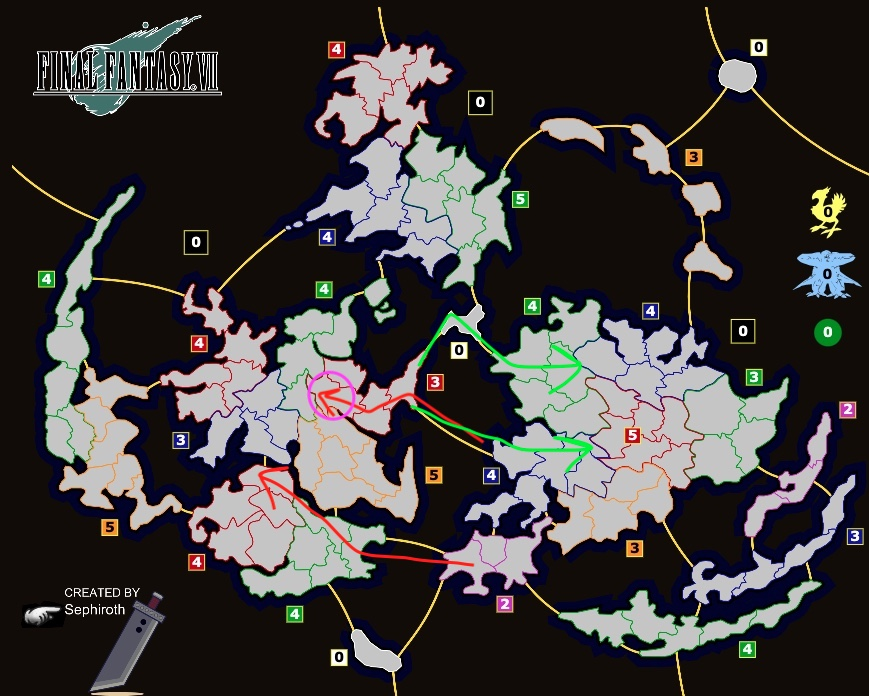
\includegraphics[width=0.8\textwidth]{Images/ff7_proximity.jpg}
  \caption{West vs East}
  \label{ff7_proximity}
\end{figure}

\begin{itemize}
    \item If I'm only on the East looking to go to the West to break my opponent's bonuses, from south it's 3 steps to a single border, from the red +3 it's 3 steps to a double border and that's IF my opponent doesn't blockade the purple circle. (Red Arrows).
    \item If I'm only on the West looking to go to the East, from the red +3 I've got a double border on 2 steps. From the Island above it 3 steps for the same. (Light Green Arrows).
\end{itemize}
